\chapter{Riduzione e Completezza}
Capitolo 8 del libro. Alcuni problemi catturano la difficoltà di un'intera classe di complessità. La logica gioca un ruolo centrale in questo fenomeno.


\section{Riduzioni}
Si vuole risolvere un problema $A$ ``simile'' al problema $B$, e si possiede un algoritmo efficiente per $B$. Si possono eseguire una serie di trasformazioni:
$$
    \underset{\text{input per }A}{x} \to \underset{\text{input per }B}{x'} \to \text{algoritmo} \to \underset{\text{output per }B}{y'} \to \underset{\text{output per }A}{y}
$$
Se una trasformazione ha una complessità molto minore del problema, la complessità rimane la stessa. In particolare, la trasformazione più interessante è quella da $x$ a $x'$, e prende il nome di \textbf{riduzione}.
\begin{definition}[Riduzione]
    Una riduzione da $L_1$ a $L_2$ è
    $$
        R:\Sigma_1^*\to\Sigma_2^* \text{ ~ tale che ~ } x\in L_1 \Leftrightarrow R(x)\in L_2
    $$
    La complessità principale deriva dall'algoritmo per decidere $L_2$.
\end{definition}
$R$ dev'essere computabile in spazio logaritmico.

\paragraph{Esempio (Riduzione)} Si consideri il Graph 3-Coloring ($L_1$): dato un grafo $G=(V,E)$, decidere se è possibile definire $Col:V\to\{r,b,y\}$ tale che se $(u,v)\in E$ allora $Col(u)\neq Col(v)$.

Si consideri SAT ($L_2$): data una formula booleana, decidere se è soddisfacibile o meno. 
$$
    R:\text{Graph 3-Coloring}\to\text{SAT}
$$
ovvero
$$
    R(G) \text{ è soddisfacibile } \Leftrightarrow~ G \text{ è 3-colorabile}
$$
Abbiamo che 
\begin{eqnarray*}
    R(G) &=& \bigwedge_{u\in V} [(r_u\lor b_u\lor y_u) \land 
    (r_u\to \lnot b_u\land \lnot y_u) \land
    (b_u\to \lnot r_u\land \lnot y_u) \land
    (y_u\to \lnot r_u\land \lnot b_u)] \land\\
    & & \bigwedge_{(u,v)\in E} [(r_u\to \lnot r_v) \land (b_u\to \lnot b_v) \land (y_u\to \lnot y_v)]
\end{eqnarray*}
Se in una macchina di Turing con I/O si ha $G$ sul nastro di input e $R(G)$ sul nastro di output, la riduzione deve utilizzare spazio logaritmico sui working tape.

\begin{definition}[$L_1\leq L_2$]
    $L_1$ può essere ridotto a $L_2$ ($L_1\leq L_2$) se esiste una riduzione $R$ da $L_1$ a $L_2$.
\end{definition}

\begin{property} ($\circ$ è la composizione di funzioni)
    \begin{eqnarray*}
        &R_1 \text{ riduzione da } L_1 \text{ a } L_2&\\
        &R_2 \text{ riduzione da } L_2 \text{ a } L_3&\\
        &\Downarrow&\\
        &R_2\circ R_1 \text{ riduzione da } L_1 \text{ a } L_3&
    \end{eqnarray*}
\end{property}
Questo significa che $L_1\leq L_2$ e $L_2\leq L_3$ implica $L_1\leq L_3$. Inoltre, $L_1\leq L_2$ significa che, in termini di complessità, $L_1$ è al più difficile di $L_2$.

\begin{definition}[Chiusura per Riduzione]
    Sia $\mathcal{C}$ una classe di complessità. $\mathcal{C}$ è chiusa per riduzione se
    $$
        L_1\leq L_2 \text{ e } L_2\in\mathcal{C} ~\Rightarrow~ L_1\in\mathcal{C}
    $$
\end{definition}
Si può dimostrare che, ad esempio, P, NP, EXP, $\mathbb{L}$, N$\mathbb{L}$, PSPACE sono tutte chiuse per riduzione. \emph{Esercizio: trovare un esempio di una classe di complessità non chiusa per riduzione.}


\section{Completezza}

\begin{definition}[Completezza di una Classe di Complessità]
    Un linguaggio $L$ è completo per una classe $\mathcal{C}$ se
    \begin{enumerate}
        \item $L\in\mathcal{C}$
        \item $\forall L'\in\mathcal{C}$, $L'\leq L$
    \end{enumerate}    
\end{definition}

\begin{center}
    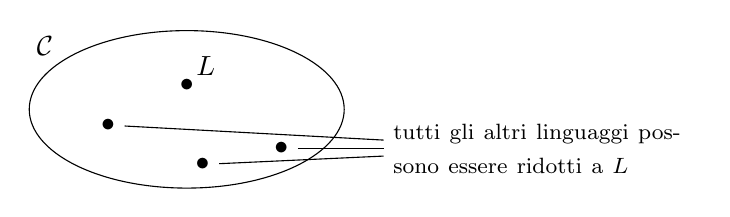
\begin{tikzpicture}
        \draw (0,0) ellipse (2 and 1);
        \node at (-1.8,0.8) {\(\mathcal{C}\)};
    
        \node (l) at (0,0.3) {$\bullet$};
        \node[above right] at (l) {$L$};

        \node (a) at (-1,-.2) {$\bullet$};
        \node (b) at (1.2,-.5) {$\bullet$};
        \node (c) at (0.2,-.7) {$\bullet$};
        \node[text width=3.8cm,right] (d) at (2.5, -.5) {\footnotesize tutti gli altri linguaggi possono essere ridotti a $L$};
        \draw (a) -- (d);
        \draw (b) -- (d);
        \draw (c) -- (d);
    \end{tikzpicture}
\end{center}

\begin{property}
    Se $\mathcal{C}$ e $\mathcal{C}'$ sono classi di complessità 
    \begin{itemize}
        \item chiuse per riduzione, e
        \item $\mathcal{C}\subseteq\mathcal{C}'$, e 
        \item $L'$ è completo per $\mathcal{C}'$, e
        \item $L'\in\mathcal{C}$
    \end{itemize}
    allora $\mathcal{C}=\mathcal{C}'$.
\end{property}

\begin{center}
    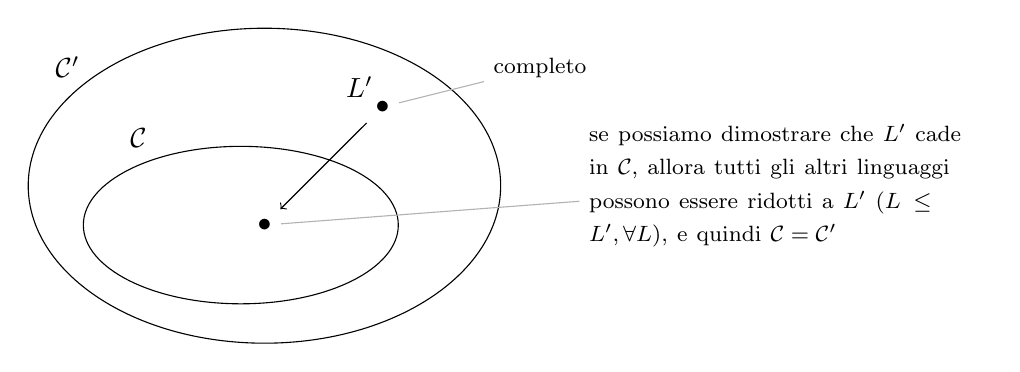
\begin{tikzpicture}
        \draw (0,0) ellipse (3 and 2);
        \node at (-2.5,1.5) {\(\mathcal{C}'\)};
        \draw (-.3,-.5) ellipse (2 and 1);
        \node at (-1.6,.6) {\(\mathcal{C}\)};

        \node (lp) at (1.5,1) {$\bullet$};
        \node[above left] at (lp) {$L'$};
        \node[] (tlp) at (3.5, 1.5) {\footnotesize completo};
        \draw[black!30] (lp) -- (tlp);

        \node (l) at (0,-.5) {$\bullet$};
        \draw[->] (lp) -- (l);

        \node[text width=5cm, right] (tl) at (4, 0) {\footnotesize se possiamo dimostrare che $L'$ cade in $\mathcal{C}$, allora tutti gli altri linguaggi possono essere ridotti a $L'$ ($L\leq L', \forall L$), e quindi $\mathcal{C}= \mathcal{C}'$};
        \draw[black!30] (l) -- (tl);
    \end{tikzpicture}
\end{center}



% LEZIONE 20
\subsection{Problema P-Completo: Circuit value}
Una \textbf{formula booleana} è coposta da variabili booleane $x_1,\dots,x_n$, da costanti $0,1$, e da operatori $\land,\lor,\lnot$. Una \textbf{funzione booleana} è 
$$
    \varphi:\{0,1\}^m\to\{0,1\}
$$

\paragraph{Esempio} m=3
$$
    \begin{rcases*}
        \varphi(\overset{x_1}{0},\overset{x_2}{0},\overset{x_3}{0})=1\\
        \varphi(0,1,0)=1\\
        \dots\\
        \varphi(1,1,1)=0
    \end{rcases*} \text{ dominio } |\{0,1\}^3|=8
$$
Questa funzione booleana ha valore 1 solo in due casi, ed è quindi equivalente alla formula booleana
$$
    (\lnot x_1\land \lnot x_2\land \lnot x_3) \lor (\lnot x_1\land 2\land \lnot x_3)
$$
Formule booleane ed espressioni booleane hanno lo stesso potere espressivo.\medskip

I \textbf{circuiti booleani} (boolean circuits) sono equivalenti a formule booleane ed espressioni booleane. Un circuito è composto da \emph{gates}, ovvero nodi di un grafo. I gates sono di tre tipi: variabili, costanti e operazioni.

\begin{center}
    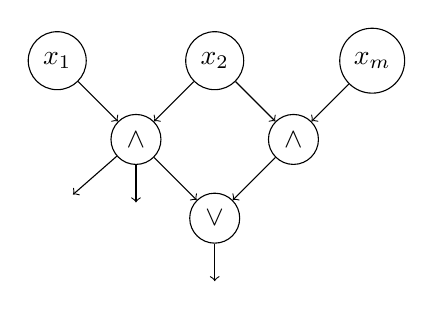
\begin{tikzpicture}
        \node[circle, draw] (x1) at (0,0) {$x_1$};
        \node[circle, draw] (x2) at (2,0) {$x_2$};
        \node[circle, draw] (xm) at (4,0) {$x_m$};
        \node[circle, draw] (and1) at (1,-1) {$\land$};
        \node[circle, draw] (and2) at (3,-1) {$\land$};
        \node[circle, draw] (or) at (2,-2) {$\lor$};

        \draw[->] (x1) -- (and1);
        \draw[->] (x2) -- (and1);
        \draw[->] (x2) -- (and2);
        \draw[->] (xm) -- (and2);
        \draw[->] (and1) -- (or);
        \draw[->] (and1) -- (1,-1.8);
        \draw[->] (and1) -- (0.2,-1.7);
        \draw[->] (and2) -- (or);
        \draw[->] (or) -- (2,-2.8);
    \end{tikzpicture}
\end{center}
Un circuito booleano è un grafo diretto aciclico nel quale un risultato può essere utilizzato più volte. Il nodo senza archi uscenti è l'output gate.

\paragraph{Circuit Value} Dato un circuito booleano $C$ senza gate con variabili, calcolare il valore di output di $C$ (o, equivalentemente, decidere se ha valore 1).\medskip

Ad esempio, il valore del seguente circuito è 1.
\begin{center}
    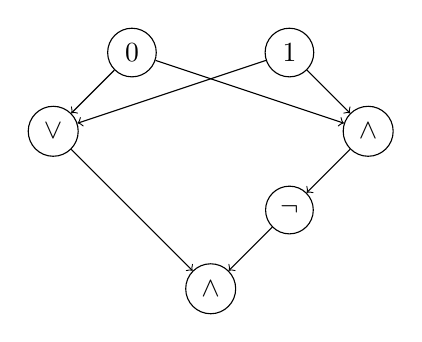
\begin{tikzpicture}
        \node[circle, draw] (x1) at (0,0) {$0$};
        \node[circle, draw] (x2) at (2,0) {$1$};
        \node[circle, draw] (or1) at (-1,-1) {$\lor$};
        \node[circle, draw] (and1) at (3,-1) {$\land$};
        \node[circle, draw] (not) at (2,-2) {$\lnot$};
        \node[circle, draw] (and2) at (1,-3) {$\land$};

        \draw[->] (x1) -- (or1);
        \draw[->] (x1) -- (and1);
        \draw[->] (x2) -- (or1);
        \draw[->] (x2) -- (and1);
        \draw[->] (or1) -- (and2);
        \draw[->] (and1) -- (not);
        \draw[->] (not) -- (and2);
    \end{tikzpicture}
\end{center}
Qual è la complessità di questo problema? Per risolverlo, si può utilizzare il topological sort, iniziando dall'output gate. Quindi Circuit Value $\in$ P.

\begin{theorem}[Cook-Levin (1)]
    Circuit Value è P-completo.
\end{theorem}

\paragraph{Dimostrazione} (pagg.~166 e seguenti) Dobbiamo dimostrare che
\begin{enumerate}
    \item Circuit Value $\in$ P $\quad \checkmark$
    \item $\forall L\in$ P, $L\leq$ Circuit Value. Si ha $L\subseteq \Sigma^*$, bisogna trovare una funzione 
    $$
        R : \Sigma^* \to \text{ circuito senza variabili t.c.~} R(x)=1 \Leftrightarrow x\in L ~\land~ R \text{ computabile in spazio } O(\log n)
    $$
    Idea: se $L\in P$, allora esiste una macchina di Turing deterministica $\mathcal{M}$ che decide $L$ in tempo $O(n^k)$.
    \begin{center}
        \begin{tikzpicture}
            \draw (0,1.5) -- (5,1.5);
            \draw (0,2) -- (5,2);
            \foreach \x in {0.5,1,1.5,3,3.5,4} {
              \draw (\x,1.5) -- (\x,2);
            }
            \node[above] at (0.75,1.5) {$\rhd$};
            \node[above] at (1.25,1.5) {$x_1$};
            \node[above] at (2.25,1.5) {\dots};
            \node[above] at (3.25,1.5) {$x_n$};
            \node[above] at (3.75,1.5) {$\sqcup$};
            \draw [decorate,
                decoration = {brace,amplitude=5pt}] (1,2.1) -- (3.5,2.1) node [midway,above=0.1] {$x$};

            \node at (1.5,1.15) {\vdots};
    
            \draw (0,.5) -- (5,.5);
            \draw (0,0) -- (5,0);
            \foreach \x in {0.5,1,1.5,2.5,3,4,4.5} {
              \draw (\x,0.5) -- (\x,0);
            }
            \node[above] at (0.75,0) {$\rhd$};
            \node[above] at (1.25,0) {$y_1$};
            \node[above] at (2,0) {\dots};
            \node[above] at (2.75,0.5) {$\substack{\text{\large $q$}\\\downarrow}$};
            \node[above] at (2.75,0) {$y_j$};
            \node[above] at (3.5,0) {\dots};
            \node[above] at (4.25,0) {$y_h$};
    
            \node at (1.5,-.5) {\vdots};

            \draw (0,-1.5) -- (5,-1.5);
            \draw (0,-1) -- (5,-1);
            \foreach \x in {0.5,1} {
              \draw (\x,-1.5) -- (\x,-1);
            }
            \node[above] at (0.75,-1.5) {$\rhd$};
            
            \node[left] at (-.2,0.25) {``foto'' intermedia $i$};
            \node[text width=4cm,right] at (8,0) {\footnotesize si vogliono ``scattare'' tante ``foto'' quante ne servono per vedere cosa succede nella computazione};
            \draw [decorate,
                decoration = {brace,amplitude=5pt}] (5.2,2) -- (5.2,-1.5) node [text width=2cm,midway,right=0.2] {almeno $n^k$ ``fotografie''};
            \draw [decorate,
                decoration = {brace,mirror,amplitude=5pt}] (1,-1.7) -- (4.5,-1.7) node [midway,below=0.2] {queste ``fotografie'' sono lunghe $n^k$};
        \end{tikzpicture}
    \end{center}
    Sia $T_\mathcal{M}(x)$ la tabella di computazione (matrice) $|x|^k\times |x|^k$ della macchina $\mathcal{M}$ sull'input $x$, con $|x|^k$ limite temporale. In questa tabella le righe sono time step, mentre le colonne sono posizioni nella stringa della macchina. La cella $T_\mathcal{M}(i,j)$ rappresenta il contenuto della posizione $j$ della stringa di $\mathcal{M}$ al time step $i$ (ovvero dopo $i$ passi della macchina). Il valore di $T_\mathcal{M}(i,j)$ dipende solo dai contenuti delle posizioni $j-1$, $j$ e $j+1$ della stringa al time step $i-1$.

    Si formano quindi delle località (\emph{locality}). Se si trova la stessa situazione in un'altra parte del nastro, si avrà lo stesso effetto (Fig.~\vref{fig:circuit}).
    % \begin{center}
    %     \begin{tikzpicture}
    %         \draw (0,1.5) -- (2.5,1.5);
    %         \draw (0,2) -- (2.5,2);
    %         \foreach \x in {0.5,1,1.5,2} {
    %           \draw (\x,1.5) -- (\x,2);
    %         }
    %         \node[above] at (0.75,1.5) {1};
    %         \node[above] at (1.25,1.5) {0};
    %         \node[above] at (1.75,1.5) {0};
    
    %         \draw (0,.5) -- (2.5,.5);
    %         \draw (0,1) -- (2.5,1);
    %         \foreach \x in {0.5,1,1.5,2} {
    %           \draw (\x,0.5) -- (\x,1);
    %         }
    %         \node[above] at (0.75,0.5) {1};
    %         \node[above] at (1.25,0.5) {1};
    %         \node[above] at (1.75,0.5) {0};
    %     \end{tikzpicture}
    % \end{center}
    \begin{figure}[htb]
        \centering
        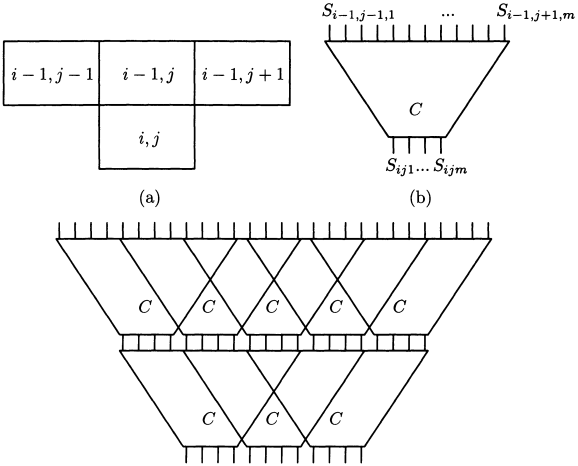
\includegraphics[width=.6\textwidth]{circuit.png}
        \caption{Costruzione del circuito.}
        \label{fig:circuit}
    \end{figure}
    I ``piccoli circuiti'' $C$ dipendono da $\mathcal{M}$, mentre l'intero circuito $C_\mathcal{M}(x)$ dipende da $\mathcal{M}$ e da $x$. $C_\mathcal{M}(x)$ può essere computato in spazio logaritmico. In particolare, poiché gli indici $i,j$ variano da 0 a $n^k$, è necessario $O(\log n^k)$ spazio per rappresentarli. \hfill$\square$
\end{enumerate}

\begin{corollary}
    $$
        L \text{ è P-completo} \quad \Leftrightarrow \quad L \in\text{P ~e~ Circuit Value} \leq L
    $$
\end{corollary}


\subsection{Problema NP-Completo: Circuit SAT}
\paragraph{Circuit SAT} Dato un circuito booleano $C$ con variabili, decidere se esiste un'assegnamento di valori $0,1$ alle variabili che rende l'output del circuito 1.

\begin{theorem}[Cook-Levin (2)]
    Circuit SAT è NP-completo.
\end{theorem}

\paragraph{Dimostrazione} Come la precedente, utilizzando però una macchina di Turing nondeterministica $\mathcal{N}$. Inoltre, ad ogni passo si hanno più scelte: si deve specificare se la scelta è 0 o 1. Si può definire una tabella $T_\mathcal{N}(x,c)$, con $c$ sequenza di scelte. Come output si ottiene un circuito $C_\mathcal{N}(x)$ con variabili, le quali arrivano dalle scelte della macchina nondeterministica. \hfill$\square$



\chapter{Problemi Completi}


\section{Problemi NP-Completi}
Dimostrare i risultati di NP-completezza è un ingrediente importante della nostra metodologia per lo studio dei problemi computazionali. Ci concentreremo su problemi NP e NP-completi. 

\subsection{SAT}
Sappiamo che Circuit SAT (SAT di formule booleane) è NP-completo. Formule booleane in CNF (conjunctive normal form) sono formule scritte come congiunzioni di disgiunzioni. Sono della forma
$$
    c_1 \land ... \land c_h
$$
dove ogni $c_i$ è una clausola, o disgiunzione di letterali. 
$$
    c_i \equiv \ell_{i,1} \lor ... \lor \ell_{i,j}
$$
Un letterale $\ell_{i,k}$ è una variabile booleana $x$ o la sua negazione $\lnot x$. Ad esempio, la formula booleana
$$
    (x_1\lor x_2\lor x_3\lor\lnot x_4) \land
    (x_2\lor x_4\lor\lnot x_5) \land
    (\lnot x_1\lor\lnot x_3\lor x_5)
$$
è in CNF. Mentre le formule in DNF sono banalmente molto semplici, quelle in CNF sono più difficili, perché si deve scegliere un letterale da ogni clausola e renderlo vero. Decidere CNF è difficile tanto quanto decidere una normale formula.
$$
    \text{SAT} \in \text{NP-completo}
$$
Solitamente con SAT ci si riferisce alla soddisfacibilità di formule in CNF.

\paragraph{3-SAT} Data la formula $\varphi$ in CNF tale che in ogni clausola ci sono al più 3 letterali, decidere se $\varphi$ è soddisfacibile. 

\begin{theorem}[NP-Completezza di 3-SAT]
    3-SAT è NP-completo.
\end{theorem}
\paragraph{Dimostrazione} Dobbiamo dimostrare che 
\begin{enumerate}
    \item 3-SAT $\in$ NP. Esiste un algoritmo nondeterministico che indovina la valutazione corretta in tempo polinomiale. $\quad \checkmark$
    \item SAT $\leq$ 3-SAT. Una generica clausola può essere mappata in una clausola con meno letterali. Prendiamo come esempio la clausola con 5 letterali 
    $$
        (x_1 \lor x_2 \lor x_3 \lor x_4 \lor x_5)
    $$
    Definiamo $z=x_1\lor x_2$. Inoltre, $z\to x_1\lor x_2\equiv \lnot z\lor(x_1\lor x_2)$. Quindi
    $$
        (z \lor x_3 \lor x_4 \lor x_5) \land (\lnot z \lor x_1 \lor x_2)
    $$
    Applicando questa tecnica più volte, si ottiene una formula con più variabili, ma ogni clause ha al più 3 letterali. \hfill$\square$
\end{enumerate}


\subsection{Caratterizzazione di NP}

\begin{definition}[Decidibile Polinomialmente]
    Una relazione binaria $R\subseteq\Sigma^*\times\Sigma^*$ è decidibile polinomialmente (deterministicamente) se, dato $(x,y)$, si può decidere in tempo $n^k$ se $(x,y)\in R$.
\end{definition}
In altre parole, $R$ è decidibile polinomialmente se esiste un algoritmo deterministico che la decide in tempo polinomiale.
\begin{definition}[Bilanciata Polinomialmente]
    Una relazione binaria $R\subseteq\Sigma^*\times\Sigma^*$ è bilanciata polinomialmente se 
    $$
        \exists h \quad \forall(x,y)\in R \quad |y|\leq |x|^h
    $$
\end{definition}

\begin{theorem}
    $L\in NP$ $\Leftrightarrow$ esiste $R$ decidibile polinomialmente e bilanciata polinomialmente t.c.~$L=\{x|\exists y~(x,y)\in R\}$
\end{theorem}
In altre parole, $y$ è un testimone, un certificato che $x\in L$. Con il certificato, si può controllare in tempo polinomiale deterministico se una soluzione è corretta.

% LEZIONE 21

\paragraph{Dimostrazione} 
\begin{itemize}
    \item[$\Rightarrow$] Se $L\in$ NP allora esiste una macchina di Turing nondeterministica $\mathcal{N}$ che decide $L$ in tempo $O(n^k)$. $\forall x\in L$, $\exists(c_1,c_2,\dots,c_{n^k})$ tali che $\mathcal{N}(x)=$ yes (ovvero insieme di scelte che produce in out\-put yes).
    $$
        R = \{ (x,y) ~|~ y=(c_1,\dots,c_{n^k}) \text{ t.c.~} \mathcal{N}^y(x)=\text{yes} \}
    $$
    con $R$ relazione binaria, $x$ stringa, $y$ stringa di interi che indica le scelte fatte. Vale che 
    $$
        L = \{ x ~|~ \exists y~(x,y)\in R \}
    $$
    poiché $\mathcal{N}$ è una macchina nondeterministica che decide $L$. La lunghezza di $y$ dev'essere polinomiale rispetto alla lunghezza di $x$ (bilanciata polinomialmente). $R$ è bilanciata polinomialmente in quanto $\mathcal{N}$ lavora in tempo polinomiale. $R$ è decidibile polinomialmente utilizzando $\mathcal{N}$ con le scelte definite da $y$.
    \item[$\Leftarrow$] Dato $x$,
    \begin{itemize}
        \item indovina $y$ di lunghezza al massimo $|x|^k$ (nondeterministico polinomiale sulla lunghezza di $x$)
        \item controlla $(x,y)\in R ~\Leftrightarrow$ tempo polinomiale 
        $$
            (|x|+|y|)^h \leq (|x| + |x|^k)^h
        $$
        (deterministico polinomiale sulla lunghezza di $x$)
    \end{itemize}
    Questi due assieme sono nondeterministici polinomiali per $L$. Invece di risolvibili efficientemente, questi problemi sono verificabili efficientemente. \hfill$\square$ 
\end{itemize}

\paragraph{NP-completezza di un linguaggio} In generale, per dimostrare che un linguaggio $L$ è NP-completo, si deve dimostrare che 
\begin{enumerate}
    \item $L\in$ NP
    \item dato un linguaggio $L''\in$ NP-completo, $\forall L''\in$ NP, $L''\leq L'$, $L'\leq L$. 
\end{enumerate}


\subsection{Independent Set}
\paragraph{Independent Set (IS)} Dato un grafo $G=(V,E)$ e un intero $k$, decidere se esiste  in $G$ un insieme di nodi $I$ tale che $|I|\geq k$ e $\forall u,v\in I$, $(u,v)\notin E$.\medskip

Dimostriamo che IS è NP-completo.
\begin{enumerate}
    \item Dati $G$ e $I$, in tempo polinomiale si può controllare $|I|\geq k$ e $\forall u,v\in I$, $(u,v)\notin E$. Quindi IS $\in$ NP.
    \item Si vuole dimostrare 3-SAT $\leq$ IS. Sia $\varphi$ la formula
    $$
        c_1\land c_2\land\dots\land c_k \equiv
        (\ell_{1,1}\lor\ell_{1,2}\lor\ell_{1,3}) \land
        (\ell_{2,1}\lor\ell_{2,2}\lor\ell_{2,3}) \land
        \dots \land
        (\ell_{k,1}\lor\ell_{k,2}\lor\ell_{k,3})
    $$
    Ad ogni letterale nella formula corrisponde un nodo nel grafo
    $$
        V = \{ \ell_{i,j} ~|~ \ell{i,j}\in\varphi \}
    $$
    I nodi sono esattamente i letterali nella formula.
    \begin{center}
        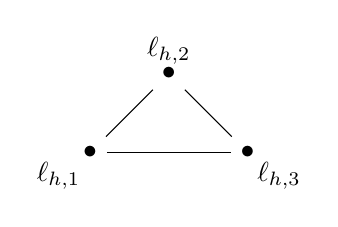
\begin{tikzpicture}
            \node[] (A) at (0,0) {$\bullet$};
            \node[] (B) at (2,0) {$\bullet$};
            \node[] (C) at (1,1) {$\bullet$};
            \node[below left] at (A) {$\ell_{h,1}$};
            \node[below right] at (B) {$\ell_{h,3}$};
            \node[above] at (C) {$\ell_{h,2}$};
            
            \draw (A) -- (B);
            \draw (B) -- (C);
            \draw (C) -- (A);
        \end{tikzpicture}
    \end{center}
    Ogni letterale è connesso alla sua negazione.
    \begin{center}
        \begin{tikzpicture}
            \node[] (A) at (0,0) {$\bullet$};
            \node[] (B) at (2,0) {$\bullet$};
            \node[] (C) at (1,1) {$\bullet$};
            \node[left=0.1] at (A) {$\lnot x$};
            \draw (A) -- (B);
            \draw (B) -- (C);
            \draw (C) -- (A);

            \node[] (D) at (-1,-2) {$\bullet$};
            \node[] (E) at (1,-2) {$\bullet$};
            \node[] (F) at (0,-1) {$\bullet$};
            \node[left=0.1] at (F) {$x$};
            \draw (D) -- (E);
            \draw (E) -- (F);
            \draw (F) -- (D);

            \node[] (G) at (3,-2) {$\bullet$};
            \node[] (H) at (5,-2) {$\bullet$};
            \node[] (I) at (4,-1) {$\bullet$};
            \node[below=0.1] at (G) {$\lnot x$};
            \draw (G) -- (H);
            \draw (H) -- (I);
            \draw (I) -- (G);

            \draw (A) -- (F);
            \draw (F) -- (G);
        \end{tikzpicture}
    \end{center}
    Controllare se $G$ ha un IS di dimensione $k$ (con $k$ numero di clausole della formula) è equivalente a controllare se $\varphi$ è soddisfacibile. 
    \begin{center}
        \begin{tikzpicture}
            \draw (0,1.5) -- (5,1.5);
            \draw (0,2) -- (5,2);
            \foreach \x in {0.5,1} {
              \draw (\x,1.5) -- (\x,2);
            }
            \node[above] at (0.75,1.5) {$\rhd$};
            \draw [decorate,
                decoration = {brace,amplitude=5pt}] (1,2.1) -- (3,2.1) node [midway,above=0.1] {$y$};

            \node at (2.5,1.1) {\vdots};
    
            \draw (0,0) -- (5,0);
            \draw (0,.5) -- (5,.5);
            \foreach \x in {0.5,1} {
              \draw (\x,0.5) -- (\x,0);
            }
            \node[above] at (0.75,0) {$\rhd$};
            \draw [decorate,
                decoration = {mirror,brace,amplitude=5pt}] (1,-.1) -- (3.45,-.1) node [midway,below=0.1] {$G$};
            \draw [decorate,
                decoration = {mirror,brace,amplitude=5pt}] (3.55,-.1) -- (4.5,-.1) node [midway,below=0.1] {$k$};
    
            \node[right] at (5.2,1.75) {input};
            \node[right] at (5.2,1) {working tapes};
            \node[right] at (5.2,0.25) {output};            
        \end{tikzpicture}
    \end{center}
    \hfill$\square$
\end{enumerate}


\subsection{Clique}

\paragraph{Clique (Cricca)} Dato un grafo $G=(V,E)$ e un intero $k$, decidere se esiste un insieme di nodi $C$ tale che $|C|\geq k$ e $\forall u,v\in C$, $(u,v)\in E$.\medskip

\begin{enumerate}
    \item Dati $G$ e $C$, in tempo polinomiale si può controllare $|C|\geq k$ e $\forall u,v\in C$, $(u,v)\in E$. Quindi Clique $\in$ NP.
    \item Si vuole dimostrare IS $\leq$ Clique. Per IS, siano $G$ il grafo e $k$ l'intero. Per Clique si costruisce un grafo $G'=(V,E')$ e $E'=\{(u,v)~|~(u,v)\notin E\}$. Esiste un independent set sse esiste una clique. \hfill$\square$
\end{enumerate}
Come esempio per il punto 2, si considerino il grafo $G$ e il suo complemento $G'$
\begin{center}
    \begin{tikzpicture}
        \node at (3,2) {$G$};
        \node[] (A) at (0,0) {$\bullet$};
        \node[] (B) at (2,0) {$\bullet$};
        \node[] (C) at (1,1) {$\bullet$};
        \node[below left=0.1] at (A) {$a$};
        \node[below right=0.1] at (B) {$b$};
        \node[above=0.1] at (C) {$c$};
        \draw (A) -- (B);
        \draw (B) -- (C);
        \draw (C) -- (A);

        \node[] (D) at (4,0) {$\bullet$};
        \node[] (E) at (6,0) {$\bullet$};
        \node[] (F) at (5,1) {$\bullet$};
        \node[below left=0.1] at (D) {$d$};
        \node[below right=0.1] at (E) {$e$};
        \node[above=0.1] at (F) {$f$};
        \draw (D) -- (E);
        \draw (E) -- (F);
        \draw (F) -- (D);

        \draw (C) -- (D);
        %%%%%%%%%%

        \node at (10,2.5) {$G'$};

        \node[] (A') at (9,2) {$\bullet$};
        \node[] (B') at (9,.5) {$\bullet$};
        \node[] (C') at (9,-1) {$\bullet$};
        \node[] (D') at (11,2) {$\bullet$};
        \node[] (E') at (11,.5) {$\bullet$};
        \node[] (F') at (11,-1) {$\bullet$};
        \node[left=0.1] at (A') {$a'$};
        \node[left=0.1] at (B') {$b'$};
        \node[left=0.1] at (C') {$c'$};
        \node[right=0.1] at (D') {$d'$};
        \node[right=0.1] at (E') {$e'$};
        \node[right=0.1] at (F') {$f'$};
        \draw (A') -- (D');
        \draw (A') -- (E');
        \draw (A') -- (F');
        \draw (B') -- (D');
        \draw (B') -- (E');
        \draw (B') -- (F');
        \draw (C') -- (E');
        \draw (C') -- (F');
    \end{tikzpicture}
\end{center}


\subsection{Isomorfismo tra Sottografi}
\paragraph{Subgraph Isomorphism (SGI)} Dati $G_1,G_2$, decidere se esiste un sottografo di $G_1$ che è isomorfo a $G_2$.\medskip 

Ad esempio, $G_2$ è isomorfo a un sottografo in $G_1$, ma $G_2'$ non è presente in $G_1$.
\begin{center}
    \begin{tikzpicture}
        \node at (1,1.6) {$G_1$};
        \node (A) at (0,0) {$\bullet$};
        \node (B) at (2,0) {$\bullet$};
        \node (C) at (1,1) {$\bullet$};
        \node (D) at (2,-1.5) {$\bullet$};
        \node (E) at (0,-1.5) {$\bullet$};
        \draw (A) -- (B);
        \draw (B) -- (C);
        \draw (C) -- (A);
        \draw (A) -- (E);
        \draw (B) -- (D);
        \draw (E) -- (D);

        \node at (5,1.6) {$G_2$};
        \node (F) at (4,0) {$\bullet$};
        \node (G) at (6,0) {$\bullet$};
        \node (H) at (5,1) {$\bullet$};
        \draw (F) -- (G);
        \draw (G) -- (H);
        \draw (H) -- (F);

        \node at (9,1.6) {$G_2'$};
        \node (I) at (8,0) {$\bullet$};
        \node (J) at (10,0) {$\bullet$};
        \node (K) at (9,1) {$\bullet$};
        \node (L) at (9,-1) {$\bullet$};
        \draw (I) -- (J);
        \draw (J) -- (K);
        \draw (K) -- (I);
        \draw (I) -- (L);
        \draw (J) -- (L);
    \end{tikzpicture}
\end{center}
Clique $\leq$ SGI: siano $G$, $k$ il grafo e l'intero per Clique. Per SGI si costruiscono i grafi $G_1=G$ e $G_2=G_k$ (grafo completo con $k$ nodi). Esiste una clique di dimensione $k$ in $G$ sse esiste un sottografo isomorfo a $G_k$ in $G$. Ad esempio, cercare una 3-clique in $G$ significa cercare un pattern del tipo 
\begin{center}
    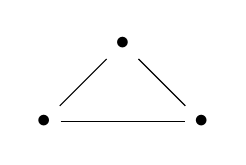
\begin{tikzpicture}
        \node (F) at (4,0) {$\bullet$};
        \node (G) at (6,0) {$\bullet$};
        \node (H) at (5,1) {$\bullet$};
        \draw (F) -- (G);
        \draw (G) -- (H);
        \draw (H) -- (F);
    \end{tikzpicture}
\end{center}



\subsection{Isomorfismo tra Grafi}
\paragraph{Graph Isomorphism (GI)} Dati $G_1,G_2$, decidere se $G_1$ è isomorfo a $G_2$.\medskip

Sappiamo che GI $\in$ NP, ma non si sa se è NP-completo. Se si dimostrasse che P $\neq$ NP, allora $\exists L$, $L\in$ NP$\backslash$P $\land$ $L\not\in$ NP-completo.



\subsection{Programmazione Intera}
\paragraph{Integer Programming (IP)} Dato un insiele di disuguaglianze lineari, decidere se esiste un assegnamento di interi alle variabili che soddisfa tutte le disuguaglianze.\medskip

3-SAT $\leq$ IP: sia $\varphi=(\ell_{1,1},\ell_{1,2},\ell_{1,3})\land(\dots)$ e ogni letterale $\ell_{i,k}$ è del tipo $p,q,r$. Per ogni variabile nella formula, consideriamo $x_p,x_{\lnot p}$. Consideriamo i seguenti vincoli per tutte le variabili nella formula
$$
\begin{cases*}
    0\leq x_p\leq 1 \\
    0\leq x_{\lnot p}\leq 1 \\
    x_p+x_{\lnot p}\geq 1 \\
    x_p+x_{\lnot p}\leq 1 \\
    \vdots \\
    x_p+x_{\lnot q}+x_r\geq 1 \\
\end{cases*}
$$
IP $\in$ NP-completo. La programmazione lineare (su $\mathbb{R}$) $\in$ P.



% LEZIONE 22
\subsection{Knapsack}
\paragraph{Knapsack} Datio $S$ insieme di oggetti, $i\in S$, con peso $w_i$ e valore $v_i$, e una sacca di peso $W$, massimizzare $V$.\medskip

Knapsack $\in$ NP-completo.

\begin{theorem}
    Ogni istanza di Knapsack può essere risolta in tempo $O(|S|W)$.
\end{theorem}
Questo è un algoritmo pseudo-polinomiale, in quanto dipende da $W$. Se fissiamo o limitiamo $W$, allora l'algoritmo è polinomiale. Tutti i problemi per i quali non esistono algoritmi pseudo-polinomiali sono detti fortemente NP-completi.



%%%%%%%%%%
\section{Problemi co-NP-Completi}

\begin{center}
    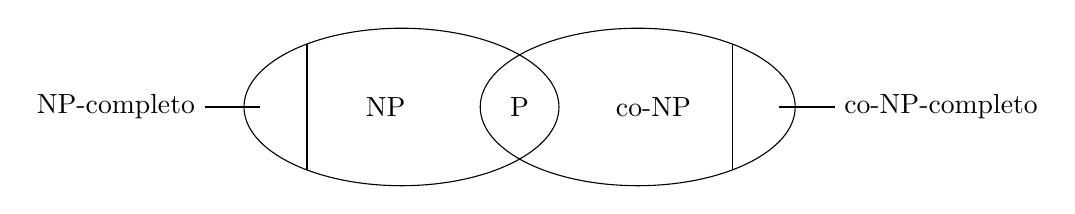
\begin{tikzpicture}
        \draw (0,0) ellipse (2cm and 1cm);
        \draw (3,0) ellipse (2cm and 1cm);
        \draw (-1.2,.8) -- (-1.2,-.8);
        \draw (4.2,.8) -- (4.2,-.8);

        \node[left] (npc) at (-2.5,0) {NP-completo};
        \node at (-.2,0) {NP};
        \node at (1.5,0) {P};
        \node at (3.2,0) {co-NP};
        \node[right] (cnpc) at (5.5,0) {co-NP-completo};
        \draw (npc) -- (-1.8,0);
        \draw (cnpc) -- (4.8,0);
    \end{tikzpicture}
\end{center}

\begin{theorem}
    $$
        L \text{ è completo per } \mathcal{C}
        \quad \Leftrightarrow \quad
        \overline{L} \text{ è completo per co-} \mathcal{C}
    $$
\end{theorem}
\paragraph{Dimostrazione} Se $L$ è completo per $\mathcal{C}$, significa che $L\in\mathcal{C}$ e $\forall L'\in\mathcal{C}$, $L'\leq L$. Quindi $\overline{L}\in$ co-$\mathcal{C}$ (definizione). Sia $L''\in$ co-N$\mathcal{C}$, allora $L''=\overline{L'}$, con $L'\in\mathcal{C}$. Sappiamo che $L'\leq L$. $L'\subseteq(\Sigma')^*$, $L\subseteq(\Sigma)^*$.
$$
    \exists R : (\Sigma')^*\to(\Sigma)^* \qquad R(x)\in L \Leftrightarrow x\in L'
$$
con $R$ computabile in spazio logaritmico. Vogliamo dimostrare che $L''\leq\overline{L}$. Si consideri $R$
$$
    x\in L'' ~\Leftrightarrow~ 
    x\not\in L' ~\Leftrightarrow~
    R(x)\not\in L ~\Leftrightarrow~
    R(x)\in\overline{L}
$$
$R$ è computabile in spazio logaritmico, quindi $L''\leq\overline{L}$. \hfill$\square$\medskip 

Ad esempio, SAT ($\forall v\dots$) è NP-completo $\Rightarrow$ UnSAT ($\exists v\dots$) è co-NP-completo.


\subsection{Validity}
\paragraph{Validity} Data una formula $\varphi$, decidere se è valida. $\varphi$ è valida sse $\lnot\varphi$ è insoddisfacibile.\medskip 

La riduzione da Validity a UnSAT si ottiene mettendo $\neg$ davanti a $\varphi$. 





%%%%%%%%%%
\section{Problemi $\mathbb{L}$-Completi}
Poiché le nostre riduzioni sono in spazio logaritmico, è difficile decidere se un linguaggio è o meno in $\mathbb{L}$. 

\begin{theorem}
    $\forall L\in\mathbb{L}$, $L\neq\emptyset$, e $L\neq\Sigma^*$, allora $L$ è $\mathbb{L}$-completo.
\end{theorem}

\paragraph{Dimostrazione} Sia $L\in\mathbb{L}$, $L\neq\emptyset$ ($x\in L$), e $L\neq\Sigma^*$ ($y\not\in L$). Sia $L'\in\mathbb{L}$
$$
    \forall x'\in L' ~ R(x')=x 
    \qquad 
    \forall x'\not\in L' ~ R(x')=y
$$
Si può dimostrare che questa riduzione è computabile in spazio logaritmico? Sì, perché $L\in\mathbb{L}$. In spa\-zio logaritmico si può decidere se $x'\in L'$, e si ottiene o $x$ o $y$.\hfill$\square$




%%%%%%%%%%
\section{Problemi N$\mathbb{L}$-Completi}

\subsection{Reachability}
Vedi il reachability method nella sezione \vref{sec:reachability}. Reachability $\in$ N$\mathbb{L}$-completo. $\forall L\in$ N$\mathbb{L}$, $\mathcal{N}$ decide $L$, $G_\mathcal{N}(x)$. Se $L\in$ N$\mathbb{L}$, allora $G_\mathcal{N}(x)$ può essere computato in spazio logaritmico.


\subsection{2-SAT}
2-SAT $\in$ N$\mathbb{L}$-completo. Abbiamo una congiunzione di clausole $c_1\land c_2\land\dots\land c_k$, dove ogni clausola è del tipo
$$
    c_i \equiv (\ell_{i,1}\lor\ell_{i,2}) \equiv (\lnot\ell_{i,1}\to\ell_{i,2}) \equiv (\lnot\ell_{i,2}\to\ell_{i,1})
$$
Queste implicazioni logiche possono essere viste come archi di un grafo.

\paragraph{Esempio} $\varphi=(x\lor\neg y)\land(\neg x\lor z)\land(\neg z\lor\neg y)$

\begin{center}
    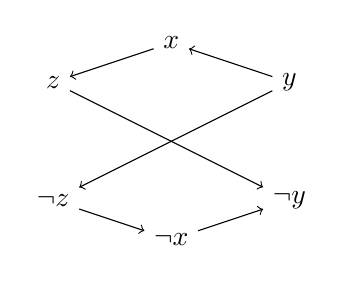
\begin{tikzpicture}
        \node (x) at (0,.5) {$x$};
        \node (nx) at (0,-2) {$\neg x$};
        \node (y) at (1.5,0) {$y$};
        \node (ny) at (1.5,-1.5) {$\neg y$};
        \node (z) at (-1.5,0) {$z$};
        \node (nz) at (-1.5,-1.5) {$\neg z$};

        \draw[->] (x) -- (z);
        \draw[->] (nx) -- (ny);
        \draw[->] (y) -- (x);
        \draw[->] (y) -- (nz);
        \draw[->] (z) -- (ny);
        \draw[->] (nz) -- (nx);
    \end{tikzpicture}
\end{center}
In questo caso $y$ raggiunge $y'$. Se, invece, prendiamo come esempio la formula 
$$
    \varphi'=(x\lor\neg y)\land(\neg x\lor z)\land(\neg z\lor\neg y)\land(y\land\neg z)\land(z\land y)
$$
\begin{center}
    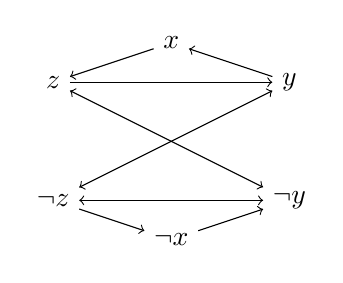
\begin{tikzpicture}
        \node (x) at (0,.5) {$x$};
        \node (nx) at (0,-2) {$\neg x$};
        \node (y) at (1.5,0) {$y$};
        \node (ny) at (1.5,-1.5) {$\neg y$};
        \node (z) at (-1.5,0) {$z$};
        \node (nz) at (-1.5,-1.5) {$\neg z$};

        \draw[->] (x) -- (z);
        \draw[->] (nx) -- (ny);
        \draw[->] (y) -- (x);
        \draw[<->] (ny) -- (z);
        \draw[<->] (ny) -- (nz);
        \draw[->] (z) -- (y);
        \draw[->] (nz) -- (nx);
        \draw[<->] (nz) -- (y);
    \end{tikzpicture}
\end{center}
Ora sia $y\to\neg y$ che $\neg y\to y$: $\varphi'$ è insoddisfacibile.





%%%%%%%%%%
% \section{Gerarchia Polinomiale}


% \textcolor{Red}{TODO: finire lezione 22}